\documentclass[12pt]{article}
\usepackage[utf8]{inputenc}
\usepackage[spanish,mexico]{babel}
%\usepackage[showframe, letterpaper]{geometry}
\usepackage[letterpaper]{geometry}
\geometry{top=1.25cm, bottom=1.0cm, left=2cm, right=2cm}
\usepackage{amsmath}
\usepackage{amsthm}
\usepackage{enumitem}
\setenumerate[1]{label=\thesection.\arabic*.}
\setenumerate[2]{label*=\arabic*.}
\usepackage{array}
\newcolumntype{C}[1]{>{\centering\arraybackslash}p{#1}}
\usepackage{caption}
\usepackage{titlesec}
%\titlespacing\section{0pt}{12pt plus 4pt minus 2pt}{0pt plus 2pt minus 2pt}
\titlespacing{\section}{0pt}{\parskip}{-\parskip}
\usepackage{multicol,multienum}
\usepackage{graphicx}
\usepackage{standalone}
\usepackage[outdir=../]{epstopdf}
\usepackage[binary-units=true]{siunitx}
\usepackage{float}
\DeclareGraphicsExtensions{.pdf,.png,.jpg}
\usepackage{tikz}
\usetikzlibrary{patterns}
\usetikzlibrary{decorations.pathmorphing,patterns}
\usetikzlibrary{arrows,calc,patterns,decorations.markings}
\usetikzlibrary{positioning}
\usepackage{color}
\usepackage{anysize}
\usepackage[spanish=mexican]{csquotes}
\usepackage{anyfontsize}
\usepackage[os=win]{menukeys}
\usepackage{pbox}
%Este paquete permite manejar los encabezados del documento
%\usepackage{fancyhdr}
%hay que definir el ambiente de la página
%\pagestyle{fancy}
%\lfoot{\small{Material elaborado por: M. en C. Gustavo Contreras Mayén \\ \hspace{4.3cm} M. en C. Abraham Lima Buendía.}}

%aqui va el texto para todas las paginas l--> izquierda, r--> derecha, hay un C--> para centrar el texto deseado
%\lhead{Curso de Física Computacional}
%\fancyhead[R]{\nouppercase{\leftmark}}
%define el ancho de la linea que separa el encabezado del cuerpo del texto
%\renewcommand{\headrulewidth}{0.5pt}
\setlength{\parskip}{1em}
\renewcommand{\baselinestretch}{1.25}
\newcommand{\python}{\texttt{python}}
\newcommand{\funcionazul}[1]{\textcolor{blue}{\textbf{\texttt{#1}}}}
\interfootnotelinepenalty=8000
\usepackage{hyperref}
%esta parte define el color del marco que aparece en las hiperreferencias.
\definecolor{links}{HTML}{2A1B81}
\hypersetup{colorlinks,linkcolor=,urlcolor=links}
\spanishdecimal{.}
\marginsize{1.5cm}{1.5cm}{1.5cm}{1.5cm}
\numberwithin{equation}{section}
\date{}
\usepackage[sfdefault]{roboto}  %% Option 'sfdefault' only if the base font of the document is to be sans serif
\usepackage[T1]{fontenc}
\title{Sistema Internacional de Medidas \\ \begin{Large}Curso de Física 2019-2\end{Large}}
%\author{M. en C. Gustavo Contreras Mayén.}
\setlength{\voffset}{-1cm}
\begin{document}
\maketitle
\vspace*{-2cm} 
\fontsize{14}{14}\selectfont
\section{Introducción.}
Al medir una cantidad, \emph{siempre la comparamos con un estándar de referencia}.
\par
El sistema de unidades empleado por los científicos en todo el mundo se denomina comúnmente \enquote{sistema métrico} aunque, desde 1960, su nombre oficial es \textbf{Sistema Internacional}, o \textbf{SI}.
\par
Son 7 unidades sobre las que se fundamenta el sistema y de cuya combinación se obtienen todas las unidades derivadas.
\par
\begin{center}
\begin{tabular}{ | c | c | c |}
\hline
Magnitud                            & Unidad    & Símbolo \\ \hline
\textbf{longitud}                   & metro     & m        \\ \hline
\textbf{masa}                       & kilogramo & kg       \\ \hline
\textbf{tiempo}                     & segundo   & s        \\ \hline
\textbf{corriente eléctrica}       & ampere    & A        \\ \hline
\textbf{temperatura termodinámica} & kelvin    & K        \\ \hline
\textbf{intensidad luminosa}        & candela   & cd       \\ \hline
\textbf{cantidad de sustancia}      & mol       & mol      \\ \hline
\end{tabular}
\end{center}
\subsection{Metro}
Es la longitud de la trayectoria recorrida por la luz en el vacío en un lapso de $1/299 792 458$ de segundo.
\subsection{Masa}
Es la masa igual a la del prototipo internacional del kilogramo: un cilindro de platino iridio de diámetro y altura iguales (39 mm)
\par
Curiosidades sobre el cilindro:
\begin{enumerate}[label=\roman*.]
\item Se fabricó en 1889.
\item La proporción de platino es del $90\%$ y $10\%$ de iridio.
\item Está resguardado en la Oficina del Buró Internacional de Pesos y Medidas (BIPM)
\item Existen sólo 6 copias oficiales.
\item Se han distribuido $80$ copias en el mundo para adaptarlas como prototipos.
\item El manejo de la campana es extremadamente cuidadoso, ya que evita el contacto con polvo, humedad, etc.
\end{enumerate}
\subsection{Segundo}
Es la duración de $9 192 631 770$ períodos de la radiación correspondiente a la transición entre los dos niveles hiperfinos del estado fundamental del átomo de cesio $133$.
\begin{figure}[H]
    \centering
    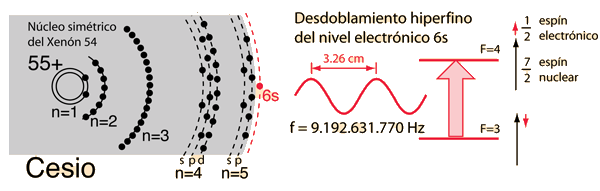
\includegraphics[scale=0.6]{./Imagenes/Csclock.png}
\end{figure}
\subsection{Ampere}
Es la intensidad de una corriente constante que mantenida en dos conductores paralelos, rectilíneos de longitud infinita, de sección circular despreciable, colocados a un metro de distancia entre sí, en el vacío, producirá entre ellos una fuerza igual a $\SI{2e-7}{\newton\per\metre}$
\subsection{Kelvin}
Es la fracción de $1/273.16$ de la temperatura termodinámica del punto triple del agua.
\par
Es de uso común expresar una temperatura termodinámica (\textbf{T}) en función de su diferencia por relación a la temperatura de referencia $T_{0} = \SI{273.15}{\kelvin}$, punto de congelación del agua.
\par
Esta diferencia de temperatura es llamada temperatura Celsius (\textbf{t}) y se define como
\[ t - T - T_{0} \]
La unidad de temperatura Celsius es el grado Celsius ($\SI{}{\celsius}$) igual a la unidad kelvin por definición.
\subsection{Candela}
Es la intensidad luminosa en una dirección dada de una fuente que emite una radiación monocromática de frecuencia $\SI{540e12}{\hertz}$ y cuya intensidad energética en esa dirección es $\SI{1/683}{\watt\per\steradian}$.
\par
Esterorradián: Se define como un ángulo sólido que, teniendo su centro en el de una esfera, tiene una superficie (sobre la esfera) igual al cuadrado del radio. El ángulo sólido de una esfera completa es $4 \: \pi$ estereorradianes.
\begin{figure}[H]
    \centering
    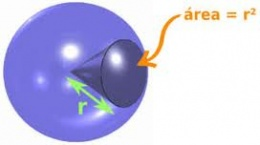
\includegraphics[scale=0.7]{./Imagenes/estereorradian.jpg}
\end{figure}
\subsection{mol}
Es la cantidad de sustancia que contiene tantas entidades elementales como existen átomos en $\SI{0.012}{\kilogram}$ de carbono $12$.
\par
En general, un mol de cualquier sustancia contiene $\num{6.022e23}$ moléculas o átomos de dicha sustancia.
\par
Así pues, en un mol de agua ($H_{2}O$) hay $\num{6.022e23}$ moléculas de $H_{2}O$. En Estados Unidos el \textcolor{blue}{día del mol} se celebra cada 23 de octubre, entre las 6:02 de la mañana y las 6:02 de la tarde aprovechando los dígitos del número de Avogadro.
\section{Unidades derivadas}
Estas unidades se forman por combinaciones simples de las unidades del SI de base de acuerdo con las leyes de la física.
\begin{center}
{\renewcommand{\arraystretch}{1.5}
\begin{tabular}{| m{5cm} | m{8cm} | c |}
\hline
\multicolumn{1}{|>{\centering\arraybackslash}m{5cm}|}{Magnitud} & Unidad SI derivada & Símbolo \\ \hline
superficie & metro cuadrado&  $\si{\square\meter}$ \\ \hline
volumen & metro cúbico & $\si{\cubic\meter}$ \\ \hline
velocidad & metro por segundo & $\si[per-mode=symbol]{\meter\per\second}$
\\ \hline
aceleración & metro por segundo al cuadrado & $\si[per-mode=symbol]{\meter\per\square\second}$ \\ \hline
densidad & kilogramo por metro cúbico & $\si[per-mode=symbol]{\kilogram\per\cubic\metre}$ \\ \hline
volumen específico & metro cúbico por kilogramo & $\si[per-mode=symbol]{\cubic\metre\per\kilogram}$ \\ \hline
densidad de corriente & ampere por metro cuadrado & $\si[per-mode=symbol]{\ampere\per\square\meter}$ \\ \hline
campo magnético & ampere por metro & $\si[per-mode=symbol]{\ampere\per\metre}$ \\ \hline
concentración (de cantidad de sustancia) & mol por metro cúbico & $\si[per-mode=symbol]{\mol\per\cubic\meter}$ \\ \hline
luminancia & candela por metro cuadrado & $\si[per-mode=symbol]{\candela\per\square\meter}$ \\ \hline
\end{tabular}
}
\end{center}
\section{Unidades derivadas con nombres y símbolos.}
Para facilitar la expresión de unidades derivadas formadas de
las combinaciones de unidades de base, se le ha dado a un cierto número de ellas un nombre y un símbolo especial.
\sisetup{detect-weight,detect-mode}
\begin{center}
{\renewcommand{\arraystretch}{1.4}
\begin{tabular}{| m{4cm} | l | c | m{4cm} | m{3cm} |}
\hline
\multicolumn{1}{|>{\centering\arraybackslash}m{4cm}|}{Magnitud} & \multicolumn{1}{|>{\centering\arraybackslash}m{3cm}|}{Nombre unidad} & \multicolumn{1}{|>{\centering\arraybackslash}m{3cm}|}{Símbolo} & \multicolumn{1}{|>{\centering\arraybackslash}m{4cm}|}{Unidades SI} &\multicolumn{1}{|>{\centering\arraybackslash}m{3cm}|}{Otra expresión SI} \\ \hline
ángulo plano & radián & \si{\radian} & \si{\meter} $\cdot$ \si{\per\meter} = 1 & \\ \hline
ángulo sólido & esterradián & \si{\steradian} & \si{\square\meter} $\cdot$ \si{\per\square\meter} = 1 & \\ \hline
frecuencia & hertz & \si{\hertz} & \si{\per\second} & \\ \hline
fuerza & newton & \si{\newton} & \si{\meter\kilogram\per\square\second} & \\ \hline
presión & pascal & \si{\pascal} & \si{\per\metre\kg\per\square\second} & \si[per-mode=symbol]{\newton\per\metre} \\ \hline
trabajo, energía, cantidad de calor & joule & \si{\joule} & \si{\meter\kilogram\per\square\second} & \si{\newton\meter} \\ \hline
potencia, flujo eléctrico & watt & \si{\watt} & \si{\meter\kilogram\per\cubic\second} & \\ \hline
carga eléctrica & coulomb & \si{\coulomb} & \si{\second\ampere} & \\ \hline 
diferencia de potencial & volt & \si{\volt} & \si{\meter\kilogram\per\cubic\second\per\ampere} & \si[per-mode=symbol]{\watt\per\ampere} \\ \hline
capacitancia eléctrica & farad & \si{\farad} & \si{\per\square\meter\per\kilogram\ampere\tothe{4}} & \si[per-mode=symbol]{\coulomb\per\ampere} \\ \hline
resistencia eléctrica & ohm & \si{\ohm} & \si{\square\meter\kilogram\cubic\second\per\square\ampere} & \si[per-mode=symbol]{\volt\per\ampere} \\ \hline
conductancia eléctrica & siemens & \si{\siemens} & \si{\per\square\meter\per\kilogram\cubic\second\square\ampere} & \si[per-mode=symbol]{\ampere\per\volt} \\ \hline
\end{tabular}
}
\end{center}


\end{document}